%==================================================
\section{Elementos finitos de orden alto}
%==================================================

\begin{contenidos}
  Elementos finitos de orden alto. Bases de Lobatto. Bases de
  Bernstein. Teoría e implementación en el ordenador.
\end{contenidos}


Para esta sección, seguiremos el TFG «Resolución Numérica de EDP
Mediante Elementos Finitos de Orden Alto y Programaciónn en Paralelo»,
del Grado en Matemáticas de la Universidad de Cádiz, presentado por
Estefanía Alonso Alonso en Julio de 2016. El PDF está
\href{https://rodin.uca.es/xmlui/bitstream/handle/10498/19255/TFG-EstefaniaAlonso.pdf}{disponible
  en el respositorio de institucional de la UCA}.
Para profundizar en el asunto, se recomienda el libro de P. \v{S}olin~\cite{solin_higher-order_2004}.

La estructura de este TFG es:
\begin{itemize}

\item \textit{Capítulo 1: Introducción a la formulación variacional de EDP}.
  Se introduce el método de Galerkin y para ello se realiza una breve
  aproximación a los espacios de Sobolev.
\item \textit{Capítulo 2: Elementos finitos nodales}. Es establecen
  las bases para el estudio del método de los elementos finitos.  Se
  plantean de forma rigurosa (en el «sentido de Ciarlet») las
  definiciones y los resultados matemáticos que son de vital
  importancia para su posterior aplicacioón. Además, de define la
  familia de elementos «clásica» conocida como elementos (nodales) de
  Lagrange.
\item \textit{Capítulo 3: Polinomios ortogonales y elementos finitos
  jerárquicos}.  Se introducen algunas familias de elementos finitos
  que mantienen buenas propiedades cuando aumenta el orden de los
  polinomios. En concreto:
  \begin{itemize}
  \item \textit{Polinomios de Legendre}, $\{L_k(x)\}_{k\ge 0}$, que
    forman una base ortogonal del espacio de Hilbert $L^2([-1,1])$.
  \item \textit{Polinomios de Lobatto}, $\{l_k(x)\}_{k\ge 0}$. Vienen
    dados (excepto para $k=0, 1$) por primitivas de polinomios de
    Legendre y por tanto sus derivadas verifican una relación de
    ortogonalidad .
  \end{itemize}
\item \textit{Capítulo 4: Implementación de elementos finitos con
    bases jerárquicas}. Se estudia la implementación en la práctica
  de elementos finitos jerárquicos (para un problema modelo
  unidimensional), analizando los pasos a seguir para su implementación
   utilizando elementos finitos continuos definidos mediante
  bases de Lobatto.
\item \textit{Capítulo 5: Experimentos numéricos}. Se pone en práctica
  todo lo anterior, en una biblioteca Fortran que utiliza elementos de
  Lagrange y de Lobatto.
 \end{itemize}

 Las conclusiones se resumen en la siguiente tabla:
 % \begin{table*}
 %   \centering
 \begin{center}
   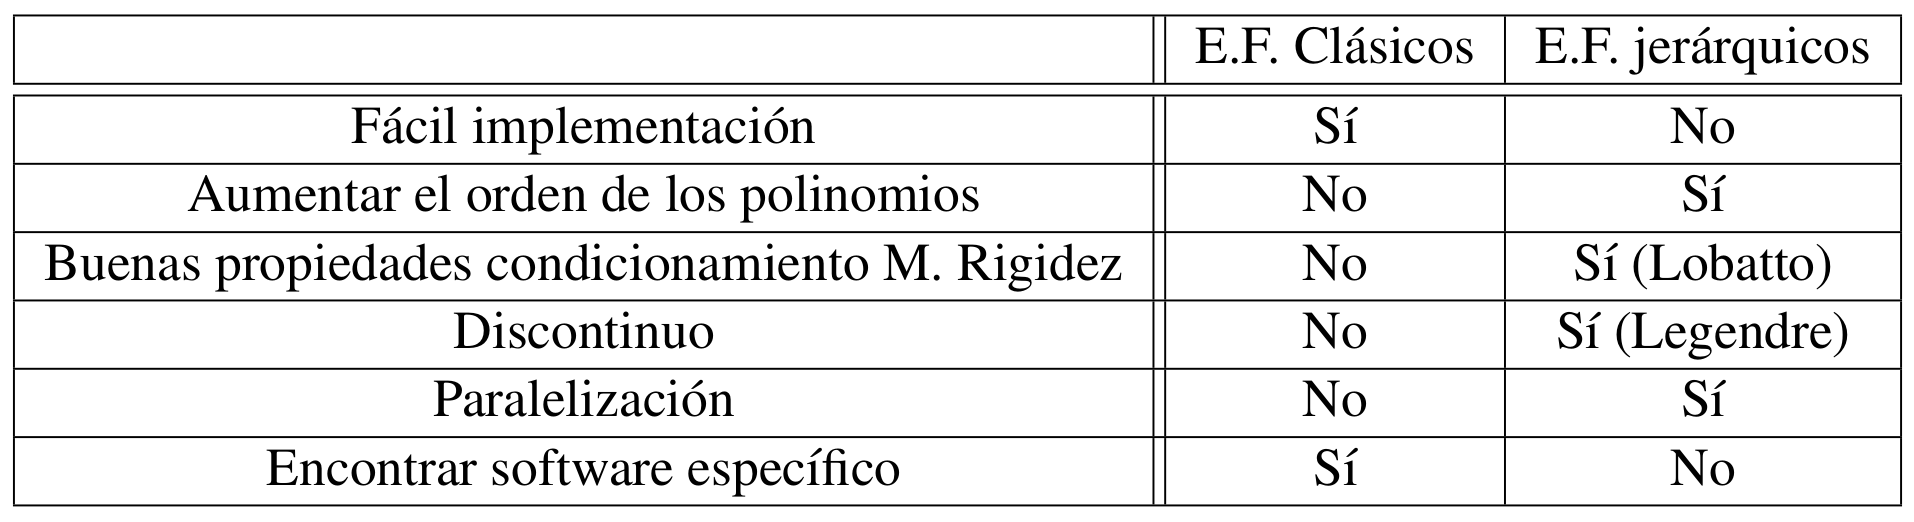
\includegraphics[width=0.75\linewidth]{img/conclusiones-bases-jerarquicas}
 \end{center}
 %   \caption{Bases jerárquicas: conclusiones}
 %   \label{tab:bases-jearquicas}
 % \end{table*}
%%% Local Variables:
%%% mode: latex
%%% TeX-master: "efavanzados.tex"
%%% End:
